\section{Modelagem}

Nesse tópicos, serão abordados os diagramas e modelagens necessários para o desenvolvimento do projeto Lixt.

\subsection{Modelo Entidade-Relacionamento (MER)}

O Modelo Entidade-Relacionamento (MER) é a primeira abstração do banco de dados, no qual é modelado e estruturado a forma no qual os dados serão trabalhados, persistidos e buscados.

\subsubsection{Apresentação do MER}

Na \autoref{fig:mer} está explicitado o MER proposto para a aplicação Lixt, sendo um diagrama normalizado e com as boas práticas aplicadas.

\begin{figure}[H]
  \centering
  \caption{Modelo Entidade-Relacionamento}
  \label{fig:mer}
  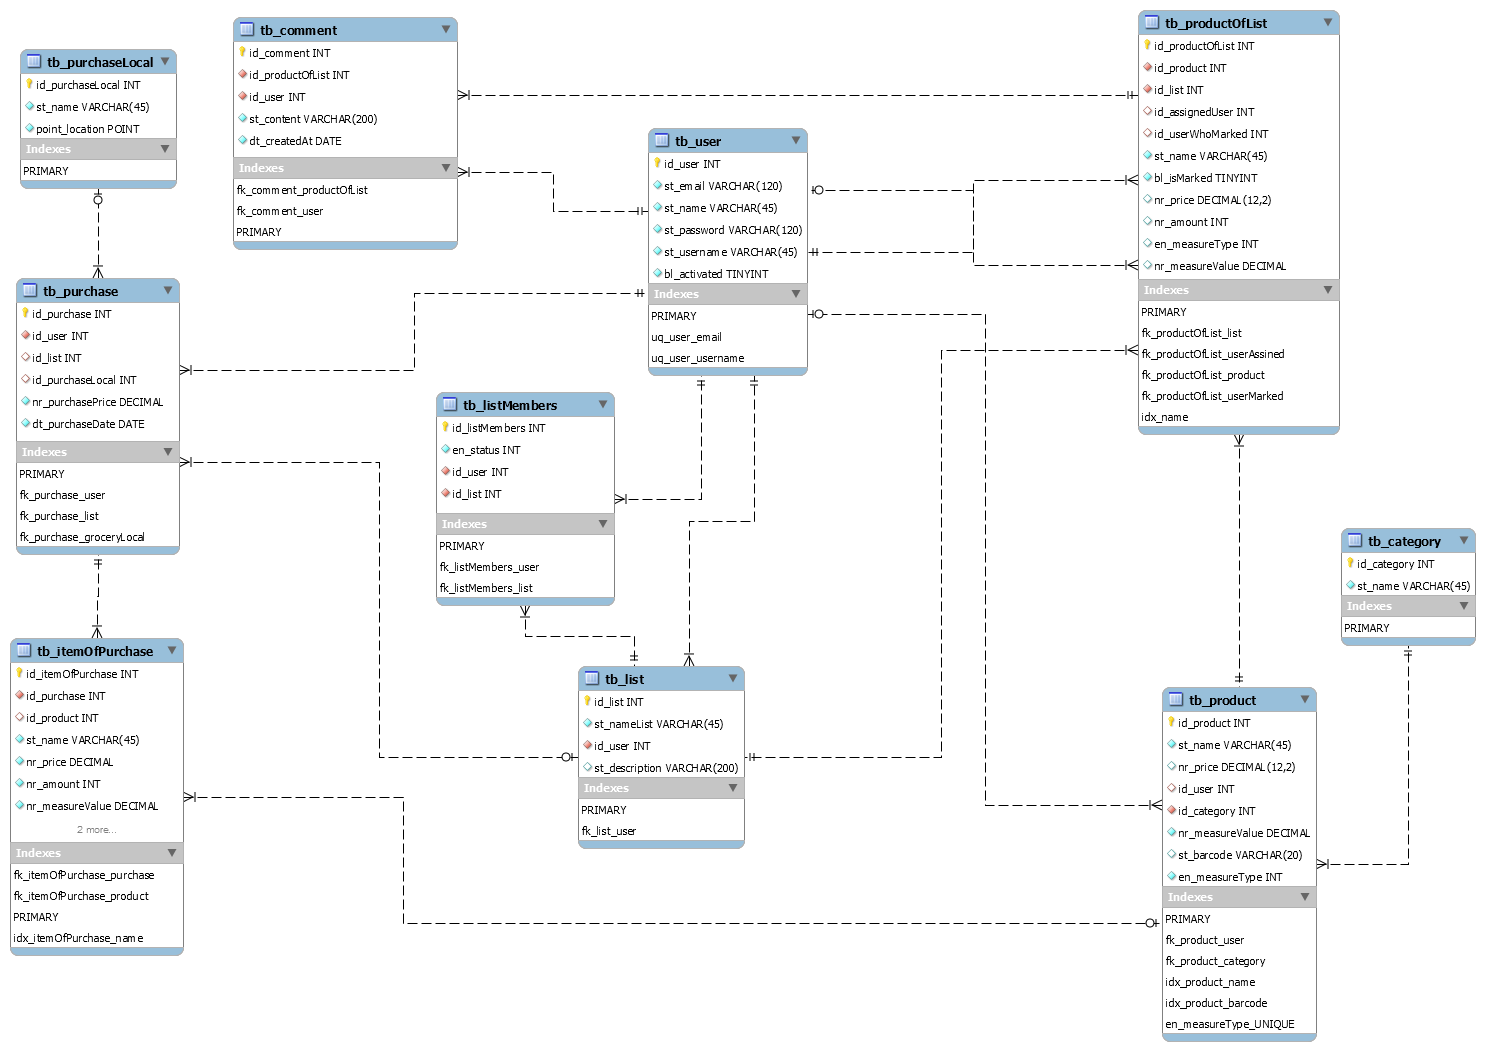
\includegraphics[scale=0.3]{mer}
  \legend{Fonte: Os autores}
\end{figure}

No diagrama, uma lista possui vários usuário, e um usuário pode estar em várias listas, surgindo assim a necessidade da tabela intermediária membrosLista. Essa tabela intermediária possui um status, que pode ser "Aceitado", "Rejeitado" e "Aguardando Confirmação".

Um cliente pode fazer vários comentários no produto da lista, 
e um comentário é de um cliente.

Uma lista pode ter várias compras (pois uma lista pode ser feita ao decorrer de várias compras), onde uma compra é de um mercado e possui vários items.

Tanto um produto da lista quanto um item da compra é 
composto um produto (sendo produto uma tabela mais genérica, pois assim será possível gerar dados estatísticos de produtos mais genéricos sem nenhuma especificidade como, por exemplo, marca do produto), sendo que o produto pode ter uma categoria.

\subsubsection{Definição de Índices}

No MySQL, temos dois tipos de índices:

\begin{enumerate}
	\item \underline{Índice Primário}: Criado pelo MySQL automaticamente ao criar chaves primárias (primary keys - PK) ou campo UNIQUE.
	\item \underline{Índice Secundário}: Criado e manipulado durante a modelagem para otimização de queries.
\end{enumerate}	

Nesse sentido, foram definidos índices secundários para as chaves estrangeiras (foreign key - FK) e para as colunas que no qual serão buscada no frontend por meio de campos de busca.

